\subsection{Projektstruktur}
Zunächst müssen die Daten in Java durch eine Datenstruktur abgebildet waren. Ich habe mich entschieden, allgemeine Eigenschaften eines Datums in einer abstrakten Oberklasse und spezifischen Unterklassen für die jeweiligen Kalendersysteme abzubilden. Hier ein UML-Diagramm:
\begin{figure}[h]
	\centering
	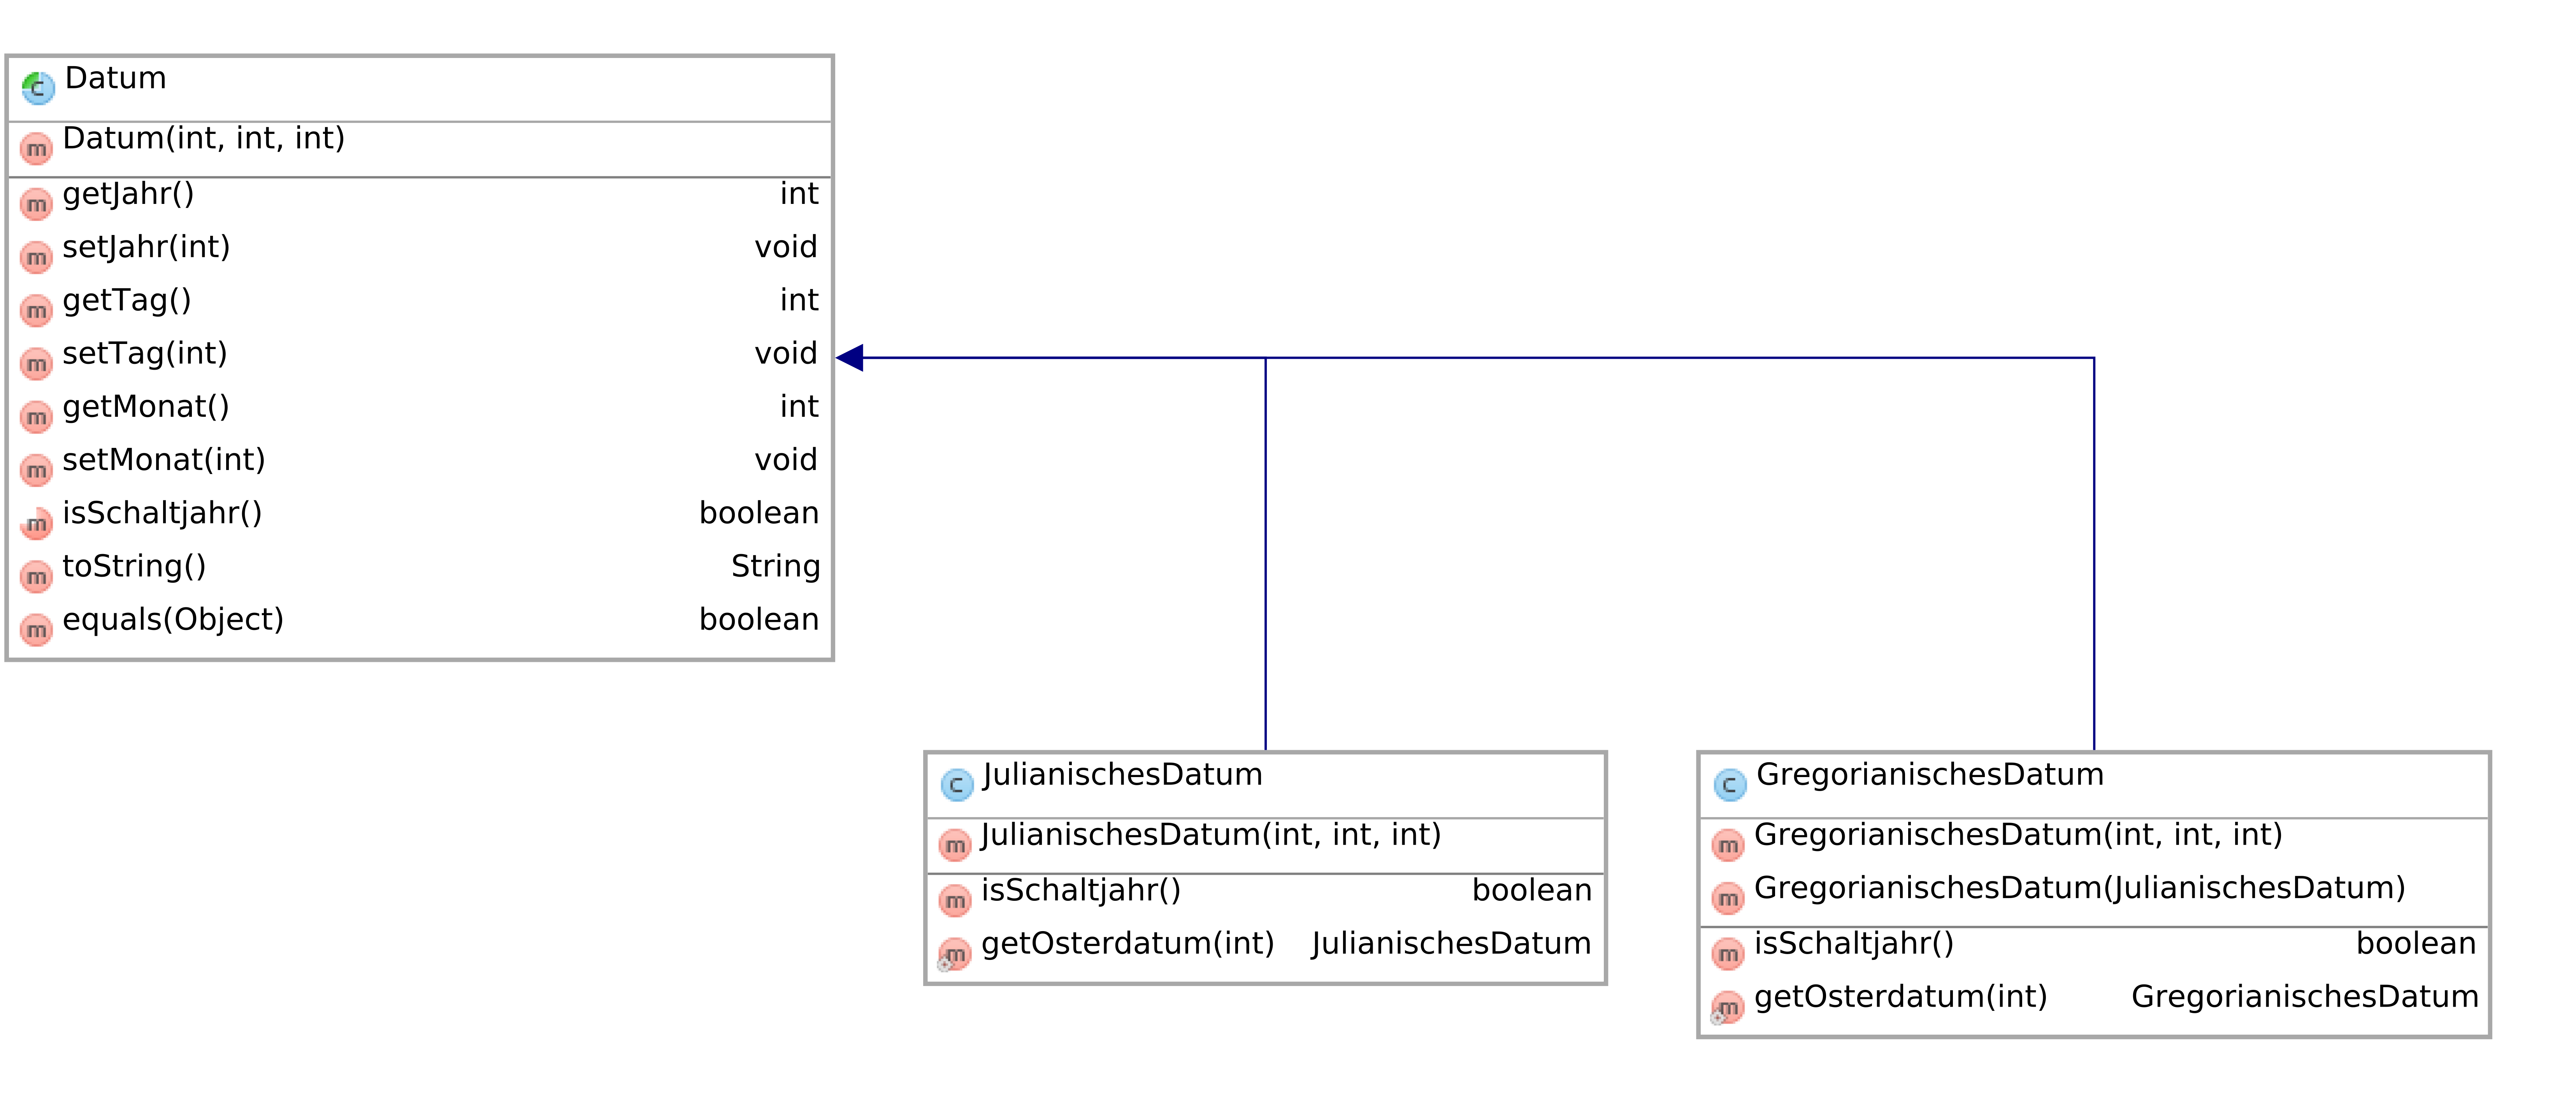
\includegraphics[width=\textwidth]{uml}
	\caption{UML-Diagramm der Implementation}
\end{figure}

Um beide Aufgabenstellungen bearbeiten zu können, muss nun für beide Kalnendersysteme getrennt die Osterformel implementiert werden. Da die Ausgabe im gregorianischen Kalendersystem gefordert wird und Daten verglichen werden müssen, müssen Daten aus dem julianischen Kalender in den gregorianischen Kalender umgerechnet werden können. Dazu gibt es in der gregorianischen Klasse einen überladenen Konstruktor, der ein julianisches Datum entgegennimmt und entsprechend umrechnet.

\clearpage
\subsection{Implementierungen der beiden Kalendersysteme}
	\subsubsection{Implementierung des julianischen Datums}
	Für die Umsetzung des julianischen Datums habe ich das obengenannte Schaltjahrkriterium folgendermaßen nach Java übersetzt:
	\lstinputlisting[firstline=9,lastline=11]{code/datum/JulianischesDatum.java}
	
	Außerdem habe ich die Osterformel von Wikipedia in Java umgesetzt:

	\lstinputlisting[firstline=13,lastline=29]{code/datum/JulianischesDatum.java}
	
	\subsubsection{Implementierung des gregorianischen Datums}

	Auch hier habe ich das Schaltjahkriterium folgendermaßen nach Java übersetzt:
	\lstinputlisting[firstline=14,lastline=16]{code/datum/GregorianischesDatum.java}
	Ebenso habe ich die für den gregorianischen Kalender angepasste Osterformel umgesetzt.
	\lstinputlisting[firstline=18,lastline=35]{code/datum/GregorianischesDatum.java}

	Außerdem gibt es in dieser Klasse noch die Umrechnungsfunktion von dem julianischen in den gregorianischen Kalender. 
	Zunächst wird dabei das julianischem Datum übernommen. Danach wird mit der in der Lösungsidee genannten Formel der Abstand zwischen den beiden Kalendersystemen in dem Jahr des Datums berechnet. Dieser Abstand wird dem Tag hinzuaddiert. Danach wird die Funktion korrigiereUeberhang() aufgerufen. Diese korrigiert das Datum falls durch das hinzuaddieren der Tagesdifferenz die Monatsläge überschritten wurde.

	Zunächst ermittelt diese Funktion die für das Jahr des Datums zutreffenden Monatslängen (Schaltjahr). Danach wird berechnet, um wie viele Tage das gesetzte Datum die Monatslänge des Datums unter-/überschreitet.

	Wenn die Monatslänge überschritten wird, wird folgendermaßen das Datum korrigiert:

	Da die Tage die Monatslänge überschritten haben, muss das Datum mindestens im nächsten Monat liegen. Daher wird der Monat des Datums um eins erhöht. Ist der aktuelle Monat ein Dezember, wird dementsprechend das Jahr um 1 erhöht, der Monat auf Januar gesetzt und der Schaltjahresregel entsprechend die für das neue Jahr gültigen Monatslängen gesetzt.

	Unterschreiten oder gleichen die überhängenden Tage die Monatslänge des neuen Monates, ist die Umrechnung beendet. Die noch überhangenden Tage sind dann der Tag des neuen Monates.

	Überschreiten die überhägenden Tage die Monatslänge des neuen Monates, wird auch dieser Monat, wie zwei Absätze zuvor beschrieben, übersprungen. Die Monatslänge kann von den überhangenden Tagen dann subtrahiert werden.

	Dies wird solange wiederholt, bis das Datum erfolgreich umgerechnet wurde.

	\lstinputlisting[firstline=36,lastline=89]{code/datum/GregorianischesDatum.java}
\clearpage
\subsection{Quelltext Suchcode}
	\lstinputlisting[firstline=14,lastline=39]{code/Main.java}